\documentclass{article}
\usepackage{amsmath}
\usepackage{amssymb}
\usepackage{tikz}
\usetikzlibrary{positioning}

\begin{document}

The induced \( P_3 \) in \( \mathcal{C}_3(P_3) \) generated by \( (\{v_1, v_3\}, C) \), for \( C = \{c_1, c_2, c_3\} \) as in Eqs.~\eqref{eq:c_example}.

\begin{center}
    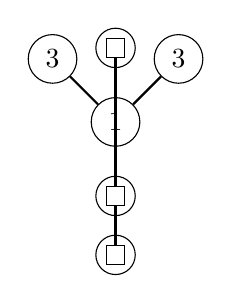
\begin{tikzpicture}[node distance=0.5cm]
        % Define nodes for the circles
        \node[circle,draw] (v1) {$1$};
        \node[circle,draw,above left=of v1] (v3) {$3$};
        \node[circle,draw,above right=of v1] (v2) {$3$};
        
        % Draw the edges between the circles
        \draw[thick] (v1) -- (v3);
        \draw[thick] (v1) -- (v2);
        
        % Define nodes for the rectangles
        \node[draw, above=of v1] (r1) {};
        \node[draw, below=of v1] (r2) {};
        \node[draw, below=of r2] (r3) {};
        
        % Draw the edges between the rectangles
        \draw[thick] (r1) -- (r2);
        \draw[thick] (r2) -- (r3);
        
        % Place the circles inside the rectangles
        \node[circle,draw,inner sep=0pt,minimum size=0.5cm,anchor=center] at (r1.center) (v1') {};
        \node[circle,draw,inner sep=0pt,minimum size=0.5cm,anchor=center] at (r2.center) (v2') {};
        \node[circle,draw,inner sep=0pt,minimum size=0.5cm,anchor=center] at (r3.center) (v3') {};
        
        % Draw the edges between the circles inside the rectangles
        \draw[thick] (v1') -- (v2');
        \draw[thick] (v2') -- (v3');
    \end{tikzpicture}
\end{center}

\end{document}